% !TEX root = ../main.tex
\begin{tikzpicture}[remember picture,overlay]
    \node[anchor=north, yshift=0.10cm] at (current page.north) {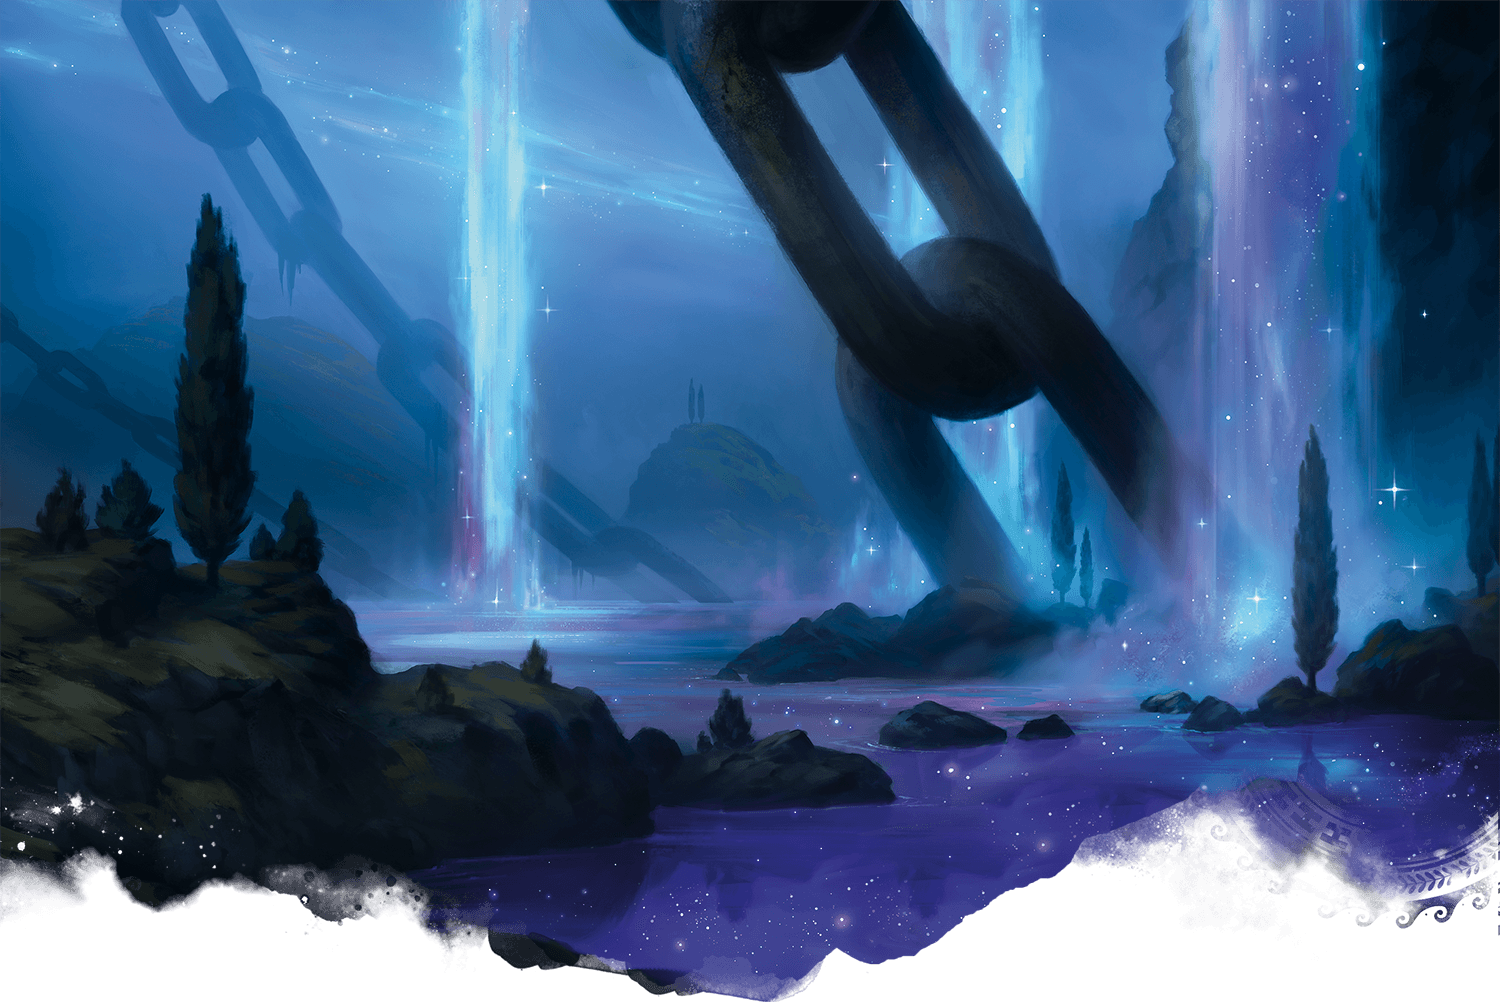
\includegraphics[width=\pdfpagewidth]{01yuadrem/img/43nyx.png}};
\end{tikzpicture}

\vspace{12.0cm}

\subsection*{Nyx}
% \DndDropCapLine{I}{f ever you find yourself beaten and}
% broke.
% And can't feel the wind for the weight of the yoke.
% And fear that the night will not turn into day.
% Remember the darkness will show you the way.
The Schism marked the beginning of an era, and with it came the opening of the Sizzling Gate.
% Through this gate spewed forth the foreigner kins, tortles, grungs, and umans.
On the other side of the portal is a strange realm, thought to be even farther from Darhoc than Thurbier.
Some even claim that this land is not even a planet at all, but an incarnation of the Cosmos itself.
This strange plane is known only as Nyx.

Nyx's topography is similar to that of Yuadrem's, its landscapes characterized by mountains, plains, ridges, etc.
Vast oceans of stars characterize the plane, fed by ever-flowing waterfalls of nebula.
Thick forests and fields of dark flora cover the shores, grazed by alien creatures known as the Nyxborn.

Titanic ruins and great, algae-slick chains rise out of the sea, as do the weathered remains of forgotten civilizations.
The sky is a misty blur of color that hangs over water as still as glass.
Mighty storms often arise from nowhere, casting souls into waves and whirlpools by the scores.

On especially dark new moons and eclipses, Nyx shows itself in the night sky, its ever-changing brilliance marked by constellations and cosmic phenomena.
Some claim that during these nights the souls of the recently dead join their ancestors in this strange land.

\pagebreak~
\vspace{13.0cm}

While Nyx is impossible to map, distinct regions do exist, and some travelers have returned to the mortal realm with tales of these incredible locations.
Each of these regions is known as a ward, and is vast beyond understanding.
Most imagine these wards as being stacked atop one another, but their actual relationships defy mortal understanding.

\subsubsection{The Tartyx River}
There is one location however that all who have traveled to Nyx claim to have seen: The Tartyx River.
The Tartyx is vast, with one far shore impossible to see from the other.
Known as the Rivers That Ring the World, it is formed from the confluence of countless tributaries from unnumbered realms.

Countless drifting islands dot the river, some forested by leafless trees, others heaped with crumpling ruins.
Still others are the domains of strange entities that death proves not quite able to claim.
None of these tiny lands are hospitable to either the living or the dead.
The waters of the Tartyx hold their own threats, both mysterious creatures that slither beneath its rippling waters, and their own infamous power to wash away memories and all sense of identity.
